% ============================================================================
% Neural Architecture Search for Function Approximation
% Duration: 35 minutes, before lunch on Day 1
% ============================================================================

\documentclass[aspectratio=169,11pt]{beamer}

% ---------- Theme and colors ----------
\usecolortheme{dove}
\setbeamertemplate{navigation symbols}{}
\setbeamertemplate{footline}{%
  \hfill\insertframenumber{}\hspace*{4pt}\vskip4pt}
\setbeamerfont{frametitle}{size=\huge}

% ---------- Packages ----------
\usepackage[utf8]{inputenc}
\usepackage[T1]{fontenc}
\usepackage{amsmath,amssymb,amsfonts}
\usepackage{bm}
\usepackage{graphicx}
\usepackage{tikz}
\usetikzlibrary{shapes,arrows.meta,positioning,calc,fit,backgrounds,patterns,decorations.pathreplacing}
\usepackage{pgfplots}
\pgfplotsset{compat=1.18}
\usepgfplotslibrary{fillbetween}
\usepackage{booktabs}
\usepackage{hyperref}
\usepackage{multicol}
\usepackage{xcolor}
\usepackage{algorithm}
\usepackage{algorithmic}

% ---------- Custom colors ----------
\definecolor{uzhblue}{rgb}{0,0,0.5}
\definecolor{uzhgreylight}{RGB}{236,238,241}
\definecolor{uzhgreydark}{RGB}{81,86,94}
\definecolor{harvardcrimson}{RGB}{153,0,0}
\definecolor{unil@blue}{RGB}{0,140,204}
\definecolor{unil@black}{RGB}{35,31,32}
\definecolor{darkgreen}{RGB}{0,100,0}
\definecolor{darkred}{RGB}{139,0,0}
\definecolor{softblue}{RGB}{70,130,180}
\definecolor{softorange}{RGB}{230,159,0}
\definecolor{softgreen}{RGB}{0,158,115}

% ---------- Set beamer colors ----------
\setbeamercolor{frametitle}{bg=uzhgreylight, fg=uzhblue}
\setbeamercolor{title}{fg=uzhblue}
\setbeamercolor{structure}{fg=uzhblue}
\setbeamercolor{block title}{bg=unil@blue, fg=white}
\setbeamercolor{block body}{bg=uzhgreylight}
\setbeamercolor{block title alerted}{bg=darkred,fg=white}
\setbeamercolor{block body alerted}{bg=red!5}
\setbeamercolor{block title example}{bg=darkgreen,fg=white}
\setbeamercolor{block body example}{bg=green!5}
\setbeamercolor{item}{fg=unil@black}
\setbeamercolor{normal text}{fg=unil@black}

% ---------- Emphasis and hyperlinks ----------
\newcommand{\emphc}[1]{\textcolor{harvardcrimson}{#1}}
\hypersetup{colorlinks,linkcolor=harvardcrimson,urlcolor=harvardcrimson}

% ---------- Math commands ----------
\newcommand{\x}{\bm{x}}
\newcommand{\w}{\bm{w}}
\newcommand{\bb}{\bm{b}}
\newcommand{\z}{\bm{z}}
\newcommand{\W}{\bm{W}}
\newcommand{\X}{\bm{X}}
\renewcommand{\a}{\bm{a}}
\newcommand{\R}{\mathbb{R}}
\newcommand{\E}[1]{\mathbb{E}\!\left[#1\right]}
\DeclareMathOperator*{\argmin}{arg\,min}
\DeclareMathOperator*{\argmax}{arg\,max}

% ---------- Title ----------
\title[NAS -- Padova 2026]%
{Deep Learning for Solving Dynamic Models}
\subtitle{Session 3a: Neural architecture search, random search and Hyperband}
\author{Simon Scheidegger}
\institute[HEC Lausanne]{HEC, University of Lausanne}
\date{University of Padova\\September 23, 2026}

\begin{document}

% ============================================================================
% TITLE
% ============================================================================

% --- Slide 1: Title ---
{\setbeamercolor{background canvas}{bg=uzhgreylight}
\begin{frame}
\titlepage
\end{frame}
}

% --- Slide 2: Roadmap ---
\begin{frame}{Roadmap of This Lecture}
\begin{columns}[T]
\column{0.48\textwidth}
\textbf{I. Motivation}
\begin{itemize}
    \item Why architecture matters
    \item The hyperparameter space
    \item Limits of manual tuning
\end{itemize}

\vspace{0.4em}
\textbf{II. Search Methods}
\begin{itemize}
    \item Grid vs.\ random search
    \item Bayesian optimization
    \item Hyperband / successive halving
    \item Method comparison
\end{itemize}

\column{0.48\textwidth}
\textbf{III. Implementing the Search}
\begin{itemize}\itemsep0pt
    \item Defining a search space
    \item Random search and successive halving from scratch
\end{itemize}

\vspace{0.4em}
\textbf{IV. Example \& Wrap-up}
\begin{itemize}\itemsep0pt
    \item Genz-function approximation
    \item The same search on a DEQN
    \item Best practices
\end{itemize}
\end{columns}

\vspace{-0.1em}
\begin{center}
{\scriptsize Hands-on, in \texttt{day1/code/03\_nas\_loss\_balancing/}:
\texttt{03\_01\_Grid\_vs\_Random\_Search.ipynb} (where to put a fixed number of trials)\\
\texttt{03\_02\_NAS\_RandomSearch\_Hyperband.ipynb} (how to spend a fixed number of epochs, and the same search on a DEQN)}
\end{center}
\end{frame}

% --- Learning objectives ---
\begin{frame}{Learning objectives}
\textbf{By the end of this lecture you should be able to:}
\begin{itemize}
  \item Measure, rather than assume, which hyperparameters move the error on a given problem
  \item State when random search beats grid search at a fixed budget, and when it does not
  \item Explain what Bayesian optimization and successive halving add to random search, and at what cost
  \item Implement random search and successive halving in plain Python, with a train / validation / test split and an exact epoch budget
  \item Run the same search on a deep equilibrium net, where the score is an Euler-equation error
\end{itemize}
\end{frame}


% ============================================================================
% PART 1: MOTIVATION
% ============================================================================

% --- Slide 3: Why Architecture Matters ---
\begin{frame}{Why Architecture Matters}
\begin{columns}[T]
\column{0.55\textwidth}
\small
\textbf{Same data, same budget, different configuration.}
Notebook \texttt{03\_02}, 30 random draws from a small search space, one smooth
two-dimensional target, 50 epochs each:
\begin{itemize}\itemsep1pt
    \item best draw: validation loss $3.2\cdot10^{-6}$
    \item hand-picked $3\times64$ ReLU, 100 epochs: $9.8\cdot10^{-6}$
    \item worst draw: $4.4\cdot10^{-2}$
\end{itemize}
4 orders of magnitude between the best and the worst draw.

\vspace{0.15cm}
\textbf{What moved it.} Notebook \texttt{03\_01}, one axis at a time: the learning rate changes
the loss by \emphc{$142\times$} over its range, the $L_2$ penalty by $1.08\times$.

\column{0.42\textwidth}
\begin{block}{The question}
Configuration choice can matter more than training time. Which knobs, and how to search them
without trying everything?
\end{block}
\vspace{0.2cm}
{\scriptsize Numbers: stored teaching runs of \texttt{03\_01} and \texttt{03\_02}, seed 0.}
\end{columns}
\end{frame}

% --- Slide 3: The Hyperparameter Space ---
\begin{frame}{The Hyperparameter Space}
\begin{columns}[T]
\column{0.50\textwidth}
\textbf{Architectural hyperparameters:}
\begin{itemize}
    \item Number of hidden layers $L \in \{1, \ldots, 5\}$
    \item Units per layer $n_\ell \in \{32, 64, \ldots, 256\}$ (8 values)
    \item Activation: ReLU, tanh, swish
\end{itemize}

\vspace{0.3cm}
\textbf{Training hyperparameters:}
\begin{itemize}
    \item Learning rate $\eta$ log-uniform on $[10^{-4}, 10^{-2}]$ (20-point grid)
    \item Batch size $B \in \{16, 32, 64, 128\}$
    \item Epochs, regularization, \ldots
\end{itemize}

\column{0.47\textwidth}
\begin{block}{Combinatorial explosion}
Even this modest search space:
\[
    |\mathcal{H}| = 5 \times 8 \times 3 \times 20 \times 4 = \emphc{9{,}600}
\]
\vspace{-0.2cm}
\begin{itemize}
    \item Each trial: minutes to hours
    \item Full grid: \emphc{infeasible}
\end{itemize}
\end{block}
\end{columns}
\end{frame}

% --- Slide 4: Manual Tuning ---
\begin{frame}{Manual Tuning}
\begin{columns}[T]
\column{0.55\textwidth}
\textbf{The ``grad-student descent'' approach:}
\begin{enumerate}
    \item Pick an architecture (intuition / paper)
    \item Train, evaluate, adjust one thing
    \item Repeat until deadline
\end{enumerate}

\vspace{0.3cm}
\textbf{Problems:}
\begin{itemize}
    \item \emphc{Doesn't scale} beyond a few hyperparameters
    \item \emphc{Human bias}: we try what we already know
    \item \emphc{Not reproducible}: results depend on the researcher
    \item Misses interactions between hyperparameters
\end{itemize}

\column{0.42\textwidth}
\vspace{0.5cm}
\begin{block}{Key insight}
We need \textbf{automated, systematic} methods to search the hyperparameter space efficiently.
\end{block}
\end{columns}
\end{frame}

% ============================================================================
% PART 2: AUTOMATED SEARCH STRATEGIES
% ============================================================================

% --- Slide 5: Section Divider ---
{\setbeamercolor{background canvas}{bg=uzhblue}
\setbeamercolor{normal text}{fg=white}
\usebeamercolor[fg]{normal text}
\begin{frame}[plain,c]
\begin{center}
{\Huge\bfseries Automated Search Strategies}
\end{center}
\end{frame}
}

% --- Slide 6: Grid Search ---
\begin{frame}{Grid Search}
\begin{columns}[T]
\column{0.52\textwidth}
\textbf{Idea:} Enumerate all combinations on a regular grid.

\vspace{0.3cm}
\begin{block}{Algorithm}
\begin{enumerate}
    \item Define discrete set for each HP
    \item Evaluate \emph{every} combination
    \item Return the best
\end{enumerate}
\end{block}

\vspace{0.2cm}
\textbf{Cost:} $\mathcal{O}(k^d)$, exponential in dimension $d$.

\vspace{0.2cm}
\textbf{Pros:} Simple, embarrassingly parallel.

\textbf{Cons:} Wastes budget on \emphc{unimportant} dimensions.

\column{0.45\textwidth}
\begin{center}
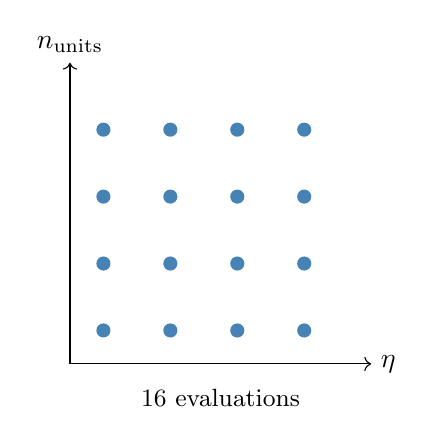
\begin{tikzpicture}[scale=0.85]
    \draw[->] (0,0) -- (4.5,0) node[right] {$\eta$};
    \draw[->] (0,0) -- (0,4.5) node[above] {$n_\text{units}$};
    % Grid points
    \foreach \xi in {0.5,1.5,2.5,3.5} {
        \foreach \yi in {0.5,1.5,2.5,3.5} {
            \fill[softblue] (\xi,\yi) circle (3pt);
        }
    }
    \node[font=\small] at (2.25,-0.5) {16 evaluations};
\end{tikzpicture}
\end{center}
\end{columns}
\end{frame}

% --- Slide 7: Random Search ---
\begin{frame}{Random Search}
\begin{columns}[T]
\column{0.52\textwidth}
\textbf{Idea:} Sample configurations uniformly at random.

\vspace{0.2cm}
\begin{block}{Key result (Bergstra \& Bengio, 2012)}
When only a \emph{few} dimensions matter, random search finds good configurations with \emphc{fewer trials} than grid search.
\end{block}

\vspace{0.2cm}
\textbf{Why?} Random points explore each dimension \emph{independently}, more unique values per HP.

\vspace{0.2cm}
\textbf{Cost:} $\mathcal{O}(n)$, linear in budget $n$.

\column{0.45\textwidth}
\begin{center}
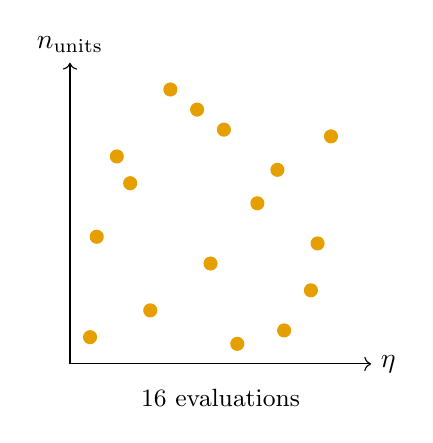
\begin{tikzpicture}[scale=0.85]
    \draw[->] (0,0) -- (4.5,0) node[right] {$\eta$};
    \draw[->] (0,0) -- (0,4.5) node[above] {$n_\text{units}$};
    % Random points (fixed seed for reproducibility)
    \fill[softorange] (0.7,3.1) circle (3pt);
    \fill[softorange] (1.2,0.8) circle (3pt);
    \fill[softorange] (2.8,2.4) circle (3pt);
    \fill[softorange] (3.6,1.1) circle (3pt);
    \fill[softorange] (0.4,1.9) circle (3pt);
    \fill[softorange] (1.9,3.8) circle (3pt);
    \fill[softorange] (3.2,0.5) circle (3pt);
    \fill[softorange] (2.1,1.5) circle (3pt);
    \fill[softorange] (0.9,2.7) circle (3pt);
    \fill[softorange] (3.9,3.4) circle (3pt);
    \fill[softorange] (1.5,4.1) circle (3pt);
    \fill[softorange] (2.5,0.3) circle (3pt);
    \fill[softorange] (3.1,2.9) circle (3pt);
    \fill[softorange] (0.3,0.4) circle (3pt);
    \fill[softorange] (2.3,3.5) circle (3pt);
    \fill[softorange] (3.7,1.8) circle (3pt);
    \node[font=\small] at (2.25,-0.5) {16 evaluations};
\end{tikzpicture}
\end{center}
\end{columns}
\end{frame}

% --- Slide 8: Grid vs Random Visual ---
\begin{frame}{Grid vs.\ Random: Why Random Wins}
\begin{center}
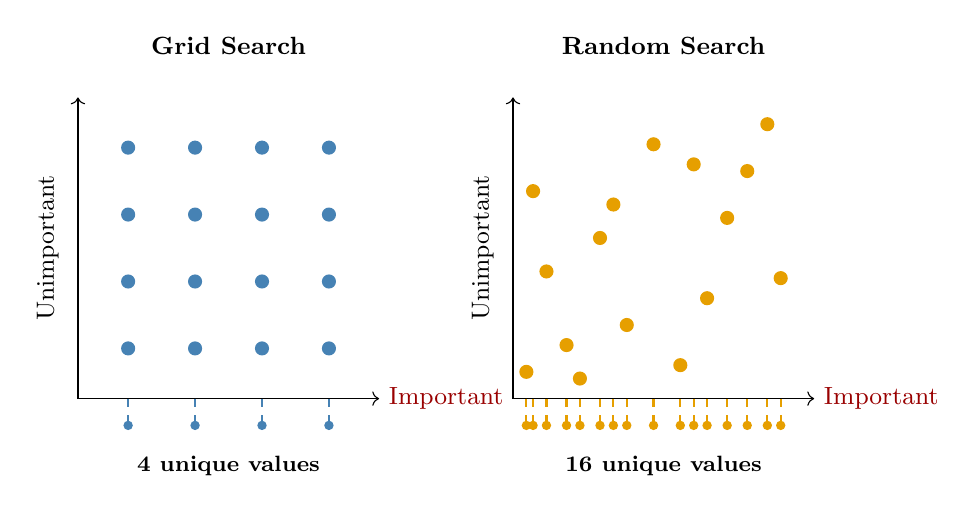
\begin{tikzpicture}[scale=0.85]
    % --- Left panel: Grid ---
    \begin{scope}[shift={(0,0)}]
        \draw[->] (0,0) -- (4.5,0) node[right,font=\small] {\emphc{Important}};
        \draw[->] (0,0) -- (0,4.5);
        \node[font=\small, rotate=90] at (-0.45,2.25) {Unimportant};
        \foreach \xi in {0.75,1.75,2.75,3.75} {
            \foreach \yi in {0.75,1.75,2.75,3.75} {
                \fill[softblue] (\xi,\yi) circle (3pt);
            }
        }
        % Project onto x-axis
        \foreach \xi in {0.75,1.75,2.75,3.75} {
            \draw[softblue, thick, dashed] (\xi,0) -- (\xi,-0.4);
            \fill[softblue] (\xi,-0.4) circle (2pt);
        }
        \node[font=\footnotesize] at (2.25,-1.0) {\textbf{4 unique values}};
        \node[font=\small, above] at (2.25,5.0) {\textbf{Grid Search}};
    \end{scope}

    % --- Right panel: Random ---
    \begin{scope}[shift={(6.5,0)}]
        \draw[->] (0,0) -- (4.5,0) node[right,font=\small] {\emphc{Important}};
        \draw[->] (0,0) -- (0,4.5);
        \node[font=\small, rotate=90] at (-0.45,2.25) {Unimportant};
        % Random points
        \fill[softorange] (0.3,3.1) circle (3pt);
        \fill[softorange] (0.8,0.8) circle (3pt);
        \fill[softorange] (1.3,2.4) circle (3pt);
        \fill[softorange] (1.7,1.1) circle (3pt);
        \fill[softorange] (0.5,1.9) circle (3pt);
        \fill[softorange] (2.1,3.8) circle (3pt);
        \fill[softorange] (2.5,0.5) circle (3pt);
        \fill[softorange] (2.9,1.5) circle (3pt);
        \fill[softorange] (3.2,2.7) circle (3pt);
        \fill[softorange] (3.5,3.4) circle (3pt);
        \fill[softorange] (3.8,4.1) circle (3pt);
        \fill[softorange] (1.0,0.3) circle (3pt);
        \fill[softorange] (1.5,2.9) circle (3pt);
        \fill[softorange] (0.2,0.4) circle (3pt);
        \fill[softorange] (2.7,3.5) circle (3pt);
        \fill[softorange] (4.0,1.8) circle (3pt);
        % Project onto x-axis
        \foreach \xi in {0.2,0.3,0.5,0.8,1.0,1.3,1.5,1.7,2.1,2.5,2.7,2.9,3.2,3.5,3.8,4.0} {
            \draw[softorange, thick, dashed] (\xi,0) -- (\xi,-0.4);
            \fill[softorange] (\xi,-0.4) circle (2pt);
        }
        \node[font=\footnotesize] at (2.25,-1.0) {\textbf{16 unique values}};
        \node[font=\small, above] at (2.25,5.0) {\textbf{Random Search}};
    \end{scope}
\end{tikzpicture}
\end{center}

\vspace{0.1cm}
{\small When one dimension matters, the grid wastes most evaluations on the
unimportant axis; random search samples the important axis more densely.}
\end{frame}

% --- Slide 8b: How big is the edge? (from 03_01) ---
\begin{frame}{How Big Is the Edge? A Measurement}
\small
\vspace{-0.15cm}
Notebook \texttt{03\_01} scores a $k^d$ grid and $k^d$ random draws on the same surface,
$v(h) = (h_1 - h^\star)^2 + \delta \sum_{i\ge2}(h_i - h^\star)^2$, 2{,}000 repetitions.
Entry $=$ grid median $/$ random median; $>1$ favours random.

\vspace{0.15cm}
\begin{center}
\renewcommand{\arraystretch}{1.1}
{\footnotesize
\begin{tabular}{@{}r rrrrrr@{}}
\toprule
$\delta$ & $d{=}1$ & $d{=}2$ & $d{=}3$ & $d{=}4$ & $d{=}5$ & $d{=}8$ \\
\midrule
0 (spare axes inert)     & 0.6 & 13 & 140 & 386 & 3{,}305 & 8{,}408 \\
0.01                     & 0.6 & 2.7 & 4.9 & 5.8 & 6.1 & 6.5 \\
0.1                      & 0.7 & 1.1 & 1.0 & 1.2 & 1.2 & 1.2 \\
1 (every axis matters)   & 0.6 & 0.6 & 0.6 & 0.7 & 0.7 & 0.8 \\
\bottomrule
\end{tabular}}
\end{center}

\vspace{0.15cm}
\begin{itemize}\itemsep1pt
  \item The edge is a statement about \emphc{dimension counting}: enormous at $d=8$, worth little at $d=2$.
  \item It needs the spare axes to be \emphc{inert}. When every axis matters, the grid wins: on one axis a grid is a stratified sample.
  \item It also needs them to be harmless. A harmful axis (dropout on a clean problem) hands the win to the grid, which always tries the endpoint (\texttt{03\_01}, Section 5).
\end{itemize}
\end{frame}

% --- Slide 9: Bayesian Optimization ---
\begin{frame}{Bayesian Optimization}
\begin{columns}[T]
\column{0.55\textwidth}
\textbf{Idea:} Build a \emph{surrogate model} of $f(\text{HP}) \to \text{loss}$ and use it to choose the next trial \emph{intelligently}.

\vspace{0.3cm}
\begin{enumerate}
    \item Fit a Gaussian process (GP) to observed trials
    \item Compute an \emphc{acquisition function} (e.g., Expected Improvement)
    \item Evaluate the HP with highest acquisition value
    \item Update the GP and repeat
\end{enumerate}

\vspace{0.3cm}
\textbf{Key advantage:} \emphc{Sample-efficient}, exploits structure in the response surface.

\column{0.42\textwidth}
\begin{block}{Expected Improvement}
\vspace{-0.2cm}
\[
    \text{EI}(\x) = \E{\max(f^* - f(\x), 0)}
\]
\vspace{-0.2cm}
\begin{itemize}
    \item $f^*$: best observed value
    \item Balances \emph{exploration} (high uncertainty) and \emph{exploitation} (low predicted loss)
\end{itemize}
\end{block}
\end{columns}
\end{frame}

% --- Slide 10: Bayesian Optimization Visual ---
\begin{frame}{Bayesian Optimization: Visual}
\begin{center}
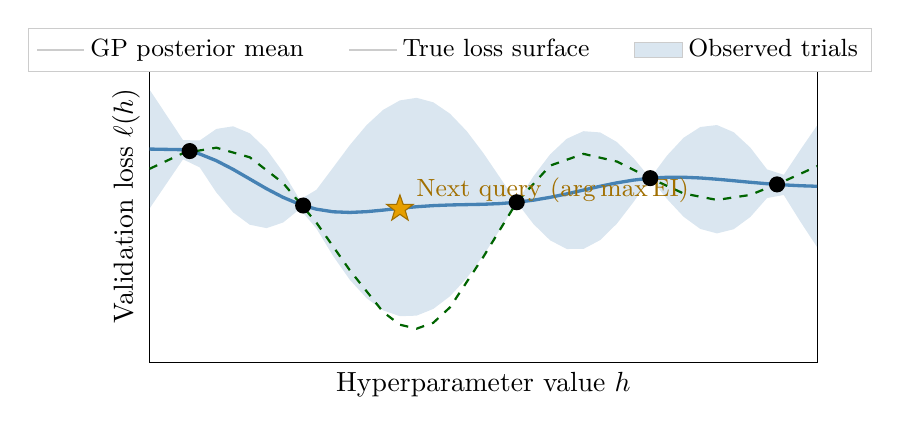
\begin{tikzpicture}[scale=0.9]
    \begin{axis}[
        width=11cm, height=6cm,
        xlabel={Hyperparameter value $h$},
        ylabel={Validation loss $\ell(h)$},
        xmin=0, xmax=10, ymin=-1.3, ymax=1.0,
        xtick=\empty, ytick=\empty,
        legend style={at={(0.5,1.03)}, anchor=south, legend columns=-1,
                      font=\small, /tikz/every even column/.append style={column sep=0.5cm},
                      draw=gray!40, fill=white},
        clip=false,
    ]
    % Uncertainty band (+-2 sigma) from a genuine RBF-GP fit
    \addplot[name path=upper, draw=none] coordinates {
      (0.000,+0.7045) (0.500,+0.3347) (0.750,+0.3315) (1.000,+0.4166) (1.250,+0.4359) (1.500,+0.3846) (1.750,+0.2677) (2.000,+0.0984) (2.250,-0.1036) (2.500,-0.0299) (2.750,+0.1338) (3.000,+0.2983) (3.250,+0.4445) (3.500,+0.5573) (3.750,+0.6262) (4.000,+0.6451) (4.250,+0.6120) (4.500,+0.5286) (4.750,+0.4008) (5.000,+0.2390) (5.250,+0.0584) (5.500,-0.1221) (5.750,+0.0683) (6.000,+0.2297) (6.250,+0.3446) (6.500,+0.4000) (6.750,+0.3908) (7.000,+0.3206) (7.250,+0.2019) (7.500,+0.0546) (7.750,+0.2200) (8.000,+0.3518) (8.250,+0.4307) (8.500,+0.4452) (8.750,+0.3927) (9.000,+0.2795) (9.250,+0.1195) (9.500,+0.0797) (9.750,+0.2634) (10.000,+0.4417)
    };
    \addplot[name path=lower, draw=none] coordinates {
      (0.000,-0.1673) (0.500,+0.1932) (0.750,+0.1339) (1.000,-0.0503) (1.250,-0.1964) (1.500,-0.2871) (1.750,-0.3122) (2.000,-0.2709) (2.250,-0.1715) (2.500,-0.3161) (2.750,-0.5179) (3.000,-0.6921) (3.250,-0.8270) (3.500,-0.9166) (3.750,-0.9591) (4.000,-0.9549) (4.250,-0.9055) (4.500,-0.8126) (4.750,-0.6796) (5.000,-0.5125) (5.250,-0.3218) (5.500,-0.1221) (5.750,-0.2819) (6.000,-0.4016) (6.250,-0.4655) (6.500,-0.4650) (6.750,-0.4000) (7.000,-0.2794) (7.250,-0.1203) (7.500,+0.0546) (7.750,-0.0971) (8.000,-0.2286) (8.250,-0.3181) (8.500,-0.3508) (8.750,-0.3205) (9.000,-0.2302) (9.250,-0.0912) (9.500,-0.0686) (9.750,-0.2648) (10.000,-0.4512)
    };
    \addplot[fill=softblue, fill opacity=0.20] fill between[of=upper and lower];

    % GP posterior mean (interpolates all 5 observations)
    \addplot[softblue, very thick] coordinates {
      (0.000,+0.2686) (0.500,+0.2640) (0.600,+0.2538) (0.750,+0.2327) (1.000,+0.1832) (1.250,+0.1197) (1.500,+0.0488) (1.750,-0.0223) (2.000,-0.0862) (2.250,-0.1375) (2.300,-0.1459) (2.500,-0.1730) (2.750,-0.1921) (3.000,-0.1969) (3.250,-0.1912) (3.500,-0.1796) (3.750,-0.1664) (4.000,-0.1549) (4.250,-0.1467) (4.500,-0.1420) (4.750,-0.1394) (5.000,-0.1368) (5.250,-0.1317) (5.500,-0.1221) (5.750,-0.1068) (6.000,-0.0859) (6.250,-0.0605) (6.500,-0.0325) (6.750,-0.0046) (7.000,+0.0206) (7.250,+0.0408) (7.500,+0.0546) (7.750,+0.0614) (8.000,+0.0616) (8.250,+0.0563) (8.500,+0.0472) (8.750,+0.0361) (9.000,+0.0246) (9.250,+0.0142) (9.400,+0.0087) (9.500,+0.0056) (9.750,-0.0007) (10.000,-0.0047)
    };
    \addlegendentry{GP posterior mean}

    % True function (hidden dip near h=4.2)
    \addplot[darkgreen, thick, dashed] coordinates {
      (0.000,+0.1238) (0.500,+0.2382) (1.000,+0.2786) (1.500,+0.2082) (2.000,+0.0189) (2.500,-0.2730) (3.000,-0.6221) (3.500,-0.9293) (3.750,-1.0217) (4.000,-1.0505) (4.250,-1.0071) (4.500,-0.8939) (5.000,-0.5230) (5.500,-0.1221) (6.000,+0.1471) (6.500,+0.2334) (7.000,+0.1771) (7.500,+0.0546) (8.000,-0.0577) (8.500,-0.1050) (9.000,-0.0681) (9.500,+0.0315) (10.000,+0.1427)
    };
    \addlegendentry{True loss surface}

    % Observed points
    \addplot[only marks, mark=*, mark size=3pt, black]
      coordinates {(0.60,+0.254) (2.30,-0.146) (5.50,-0.122) (7.50,+0.055) (9.40,+0.009)};
    \addlegendentry{Observed trials}

    % Next query: EI peak at h = 3.75 (picked from the same GP)
    \node[star, star points=5, star point ratio=2.5, fill=softorange, draw=softorange!70!black,
          minimum size=10pt, inner sep=0pt] at (axis cs:3.75,-0.17) {};
    \node[font=\small, softorange!70!black, above right] at (axis cs:3.85,-0.20) {Next query ($\arg\max\mathrm{EI}$)};
    \end{axis}
\end{tikzpicture}
\end{center}

\vspace{-0.2em}
\small The GP posterior mean \emph{interpolates} the five observations and is \emph{wide} in unexplored gaps.  The Expected-Improvement acquisition function peaks at $h \approx 3.75$, trading off the high posterior variance there against the moderately low predicted mean.
\end{frame}

% --- Slide 11: Successive halving and Hyperband ---
\begin{frame}{Successive Halving and Hyperband}
\begin{columns}[T]
\column{0.50\textwidth}
\footnotesize
\textbf{Idea:} start many configurations cheaply, \emphc{stop the worst early}, give the budget to the survivors.

\vspace{0.05cm}
\begin{block}{Successive halving (SHA), $\eta=3$}
\begin{enumerate}\itemsep0pt
    \item Draw $n$ random configurations, train each for $b$ epochs
    \item Keep the best $1/\eta$, discard the rest
    \item Budget $\times\,\eta$; \emph{continue training} the survivors
    \item Repeat until one is left
\end{enumerate}
\end{block}

\vspace{0.05cm}
\textbf{Hyperband} (Li et al., 2018): several SHA brackets with different $(n, b)$, a hedge
against the unknown correlation between early and late performance.

\column{0.48\textwidth}
\begin{center}
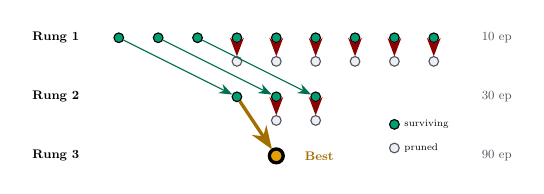
\begin{tikzpicture}[
    trialnode/.style={circle, draw, minimum size=7pt, inner sep=0pt},
    alive/.style={trialnode, fill=softgreen},
    dead/.style={trialnode, fill=uzhgreylight, draw=uzhgreydark},
    >=Stealth, scale=0.5, transform shape,
]
    \node[font=\small\bfseries] at (-1.6, 0) {Rung 1};
    \node[font=\small\bfseries] at (-1.6,-1.5) {Rung 2};
    \node[font=\small\bfseries] at (-1.6,-3.0) {Rung 3};
    \node[font=\small, uzhgreydark] at (9.6, 0) {10 ep};
    \node[font=\small, uzhgreydark] at (9.6,-1.5) {30 ep};
    \node[font=\small, uzhgreydark] at (9.6,-3.0) {90 ep};
    \foreach \i in {0,...,8} { \node[alive] (r1-\i) at (\i*1.0, 0) {}; }
    \foreach \i in {0,...,2} { \node[alive] (r2-\i) at (\i*1.0 + 3.0, -1.5) {}; }
    \foreach \i in {3,...,8} {
        \node[dead] (r1d-\i) at (\i*1.0, -0.6) {};
        \draw[->, darkred, thick] (r1-\i) -- (r1d-\i);
    }
    \draw[->, softgreen!70!black] (r1-0) -- (r2-0);
    \draw[->, softgreen!70!black] (r1-1) -- (r2-1);
    \draw[->, softgreen!70!black] (r1-2) -- (r2-2);
    \node[alive, fill=softorange, minimum size=10pt, line width=1.2pt] (r3-0) at (4.0, -3.0) {};
    \foreach \i in {1,2} {
        \node[dead] (r2d-\i) at (\i*1.0 + 3.0, -2.1) {};
        \draw[->, darkred, thick] (r2-\i) -- (r2d-\i);
    }
    \draw[->, softorange!70!black, line width=1.2pt] (r2-0) -- (r3-0);
    \node[font=\small\bfseries, softorange!70!black, right] at (4.6,-3.0) {Best};
    \node[alive, label={right:\scriptsize surviving}] at (7.0, -2.2) {};
    \node[dead, label={right:\scriptsize pruned}] at (7.0, -2.8) {};
\end{tikzpicture}
\end{center}
{\scriptsize One bracket, $9 \to 3 \to 1$ at $10 \to 30 \to 90$ epochs: $9\cdot10 + 3\cdot20 + 1\cdot60 = \emphc{210}$ epochs with continuation, against $810$ for training all nine to the end. The rung budgets add up only if survivors keep their weights between rungs.}
\end{columns}
\end{frame}

% --- Slide 13: Method Comparison ---
\begin{frame}{Method Comparison}
\begin{center}
\renewcommand{\arraystretch}{1.3}
{\small
\begin{tabular}{@{}lcccc@{}}
\toprule
\textbf{Property} & \textbf{Grid} & \textbf{Random} & \textbf{Bayesian} & \textbf{Hyperband} \\
\midrule
Computational cost & $\mathcal{O}(k^d)$ & $\mathcal{O}(n)$ & $\mathcal{O}(n)$ & $\mathcal{O}(n \log n)$ \\
Sample efficiency & Low & Medium & \emphc{High} & High \\
Parallelisable & Fully & Fully & Limited & Partially \\
Handles interactions & No & Partially & \emphc{Yes} & As random \\
Early stopping & No & No & No & \emphc{Yes} \\
Implementation & Trivial & Trivial & Moderate & Moderate \\
\bottomrule
\end{tabular}
}
\end{center}

\vspace{-0.05cm}
\textbf{Practical advice:}
\begin{itemize}
    \item \textbf{First pass:} random search, several seeds, log-scale on the learning rate. It is the baseline every other method has to beat.
    \item \textbf{Each trial is expensive and sequential is fine:} Bayesian optimization.
    \item \textbf{Bad trials show early:} successive halving or Hyperband; count the budget in epochs, and continue survivors rather than restarting them.
\end{itemize}
\end{frame}

% ============================================================================
% PART 3: IMPLEMENTING THE SEARCH (FROM SCRATCH)
% ============================================================================

% --- Slide 14: Section Divider ---
{\setbeamercolor{background canvas}{bg=uzhblue}
\setbeamercolor{normal text}{fg=white}
\usebeamercolor[fg]{normal text}
\begin{frame}[plain,c]
\begin{center}
{\Huge\bfseries Implementing the Search}\\[0.3cm]
{\large\itshape Random Search and Successive Halving, from scratch}
\end{center}
\end{frame}
}

% --- Slide 15: Defining a Search Space (plain Python) ---
\begin{frame}[fragile]{Defining a Search Space}
\begin{block}{A plain dict, no library required}
{\scriptsize
\begin{verbatim}
SPACE = {
    "layers":     [1, 2, 3, 4, 5],
    "units":      [32, 64, 96, 128, 160, 192, 224, 256],
    "activation": ["relu", "tanh", "swish"],
    "lr":         ("log_uniform", 1e-4, 1e-1),
}
def sample_config(rng):
    return {
        "layers":     int(rng.choice(SPACE["layers"])),
        "units":      int(rng.choice(SPACE["units"])),
        "activation": str(rng.choice(SPACE["activation"])),
        "lr":         float(10 ** rng.uniform(-4, -1)),
    }
\end{verbatim}
}
\end{block}
{\scriptsize The search space is a dict, the sampler is one function. The learning-rate range reaches $10^{-1}$ because \texttt{03\_01} found the optimum near $10^{-2}$; a range that stops there puts the best region on the boundary.}
\end{frame}

% --- Slide 16: Random Search from scratch ---
\begin{frame}[fragile]{Random Search from Scratch}
\begin{block}{30 trials, one function}
{\scriptsize
\begin{verbatim}
def random_search(n_trials=30, epochs=50, seed=0):
    rng, records = np.random.default_rng(seed), []
    for t in range(n_trials):
        cfg   = sample_config(rng)
        model = build_model(cfg)
        h = model.fit(X_train, y_train, epochs=epochs,
                      validation_data=(X_val, y_val), verbose=0)
        records.append((cfg, min(h.history["val_loss"])))
    return min(records, key=lambda r: r[1])   # ranked on validation
\end{verbatim}
}
\end{block}
{\scriptsize Independent uniform draws; cost exactly $N \cdot R$ epochs, embarrassingly parallel (Bergstra \& Bengio, 2012). Three sets: the search ranks on \texttt{X\_val}; \texttt{X\_test} is touched once, by the winner.}
\end{frame}

% --- Slide 17: Successive Halving from scratch ---
\begin{frame}[fragile]{Successive Halving from Scratch}
\vspace{-0.15cm}
\begin{block}{$n_0=27$, $\eta=3$, three rungs, survivors continue}
{\scriptsize
\begin{verbatim}
def successive_halving(n0=27, eta=3, r0=8, rounds=3, seed=0):
    rng   = np.random.default_rng(seed)
    alive = [dict(cfg=c, model=build_model(c), trained=0)
             for c in (sample_config(rng) for _ in range(n0))]
    target = r0
    for k in range(rounds):
        for a in alive:                         # pay only the extra epochs
            a["val"] = fit_epochs(a["model"], target - a["trained"])
            a["trained"] = target
        alive.sort(key=lambda a: a["val"])
        alive  = alive[:max(1, len(alive) // eta)] if k < rounds-1 else alive[:1]
        target *= eta                           # 8 -> 24 -> 72 epochs
    return alive[0]
\end{verbatim}
}
\end{block}
{\scriptsize Schedule: 27 at 8 epochs $\to$ 9 continued to 24 $\to$ 3 continued to 72 $\to$ 1 winner. Epochs paid: $27\cdot 8 + 9\cdot 16 + 3\cdot 48 = 504$, against $1500$ for 30 random-search trials at 50 epochs. Libraries (KerasTuner, Optuna, Ray Tune) wrap these same loops; the algorithms outlive the APIs.}
\end{frame}

% ============================================================================
% PART 4: EXAMPLE --- GENZ FUNCTION APPROXIMATION
% ============================================================================

% --- Slide 19: Section Divider ---
{\setbeamercolor{background canvas}{bg=uzhblue}
\setbeamercolor{normal text}{fg=white}
\usebeamercolor[fg]{normal text}
\begin{frame}[plain,c]
\begin{center}
{\Huge\bfseries Example: Genz Function}\\[0.3cm]
{\Large\bfseries Approximation}
\end{center}
\end{frame}
}

% --- Slide 20: Setup ---
\begin{frame}{Experiment Setup}
\begin{columns}[T]
\column{0.52\textwidth}
\textbf{Target function:} Genz Gaussian on $[0,1]^2$
\[
    f(\x) = \exp\!\Bigl(-\sum_{i=1}^{d} c_i^2 (x_i - w_i)^2\Bigr)
\]

\vspace{0.2cm}
\textbf{Data:}
\begin{itemize}
    \item $d = 2$, uniform random samples
    \item train $1{,}000$, validation $1{,}000$, test $2{,}000$
    \item Loss: MSE; trials ranked on validation loss
\end{itemize}

\column{0.45\textwidth}
\textbf{Search space:}
\begin{itemize}
    \item Layers: $1$--$5$
    \item Units/layer: $32$--$256$ (step 32)
    \item Activation: ReLU, tanh, swish
    \item LR: $10^{-4}$--$10^{-1}$ (log scale)
\end{itemize}

\vspace{0.3cm}
\textbf{Baseline:} $3 \times 64$ ReLU MLP, $\eta = 10^{-3}$, 100 epochs

\vspace{0.2cm}
\textbf{Budget:} random search $30 \times 50 = 1500$ epochs; SHA $504$ epochs; three seeds each
\end{columns}
\end{frame}

% --- Slide 21: Search Results ---
\begin{frame}{Search Results on the Genz Gaussian}
\begin{center}
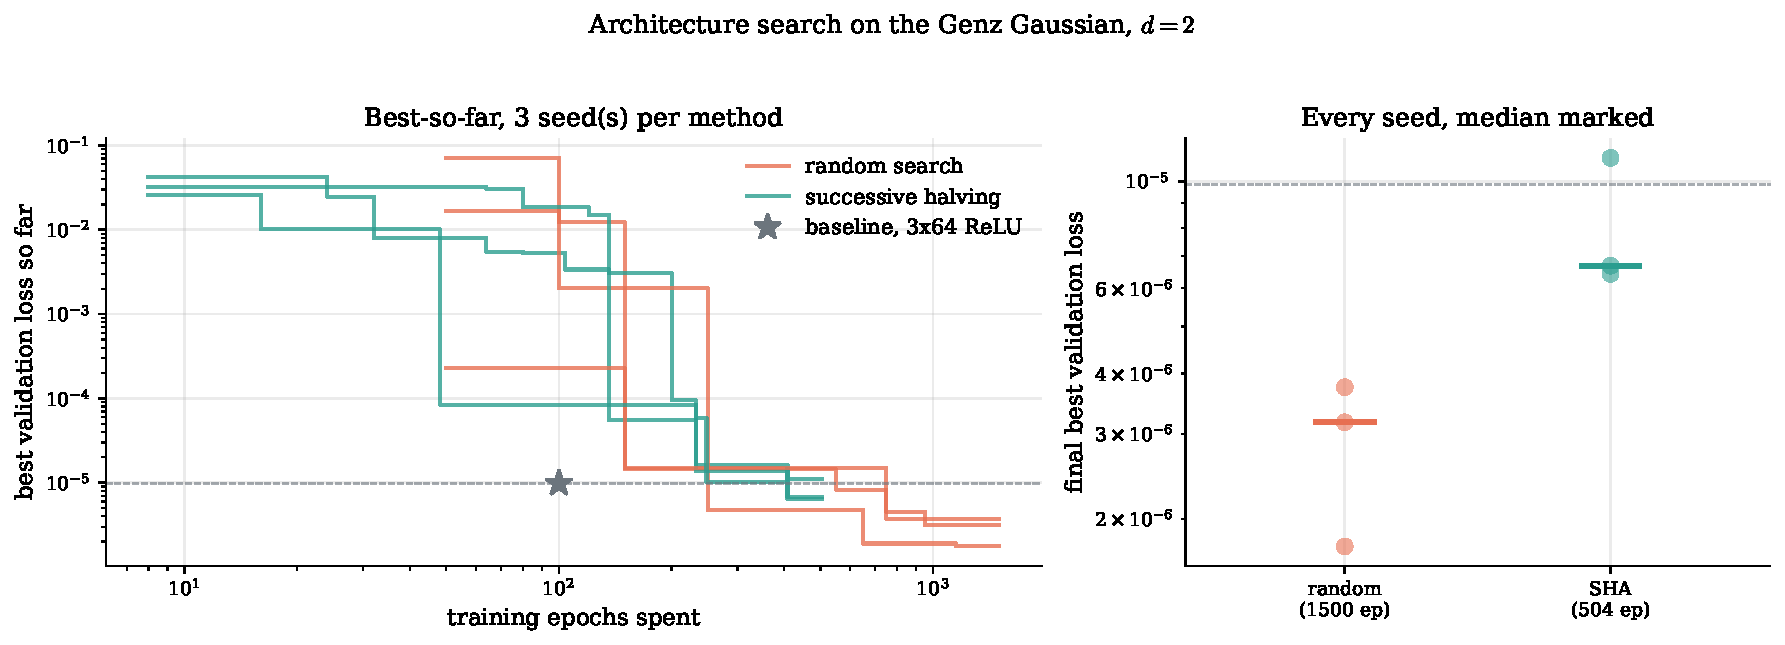
\includegraphics[width=0.88\linewidth]{figures/nas_search_results.pdf}
\end{center}

\vspace{-0.4em}
{\scriptsize Stored teaching run of \texttt{03\_02}, three seeds per method, horizontal axis in epochs paid. Median best validation loss: random search $3.2\cdot10^{-6}$ at 1500 epochs, SHA $6.7\cdot10^{-6}$ at 504 epochs, baseline $9.8\cdot10^{-6}$ at 100. Random search is ahead on all three seeds and the ranges do not overlap (random $1.8\cdot10^{-6}$ to $3.7\cdot10^{-6}$, SHA $6.4\cdot10^{-6}$ to $1.1\cdot10^{-5}$), SHA got within a factor of two for a third of the epochs.}
\end{frame}

% --- Slide 22: Visualization ---
\begin{frame}{Best Model vs.\ Ground Truth}
\begin{center}
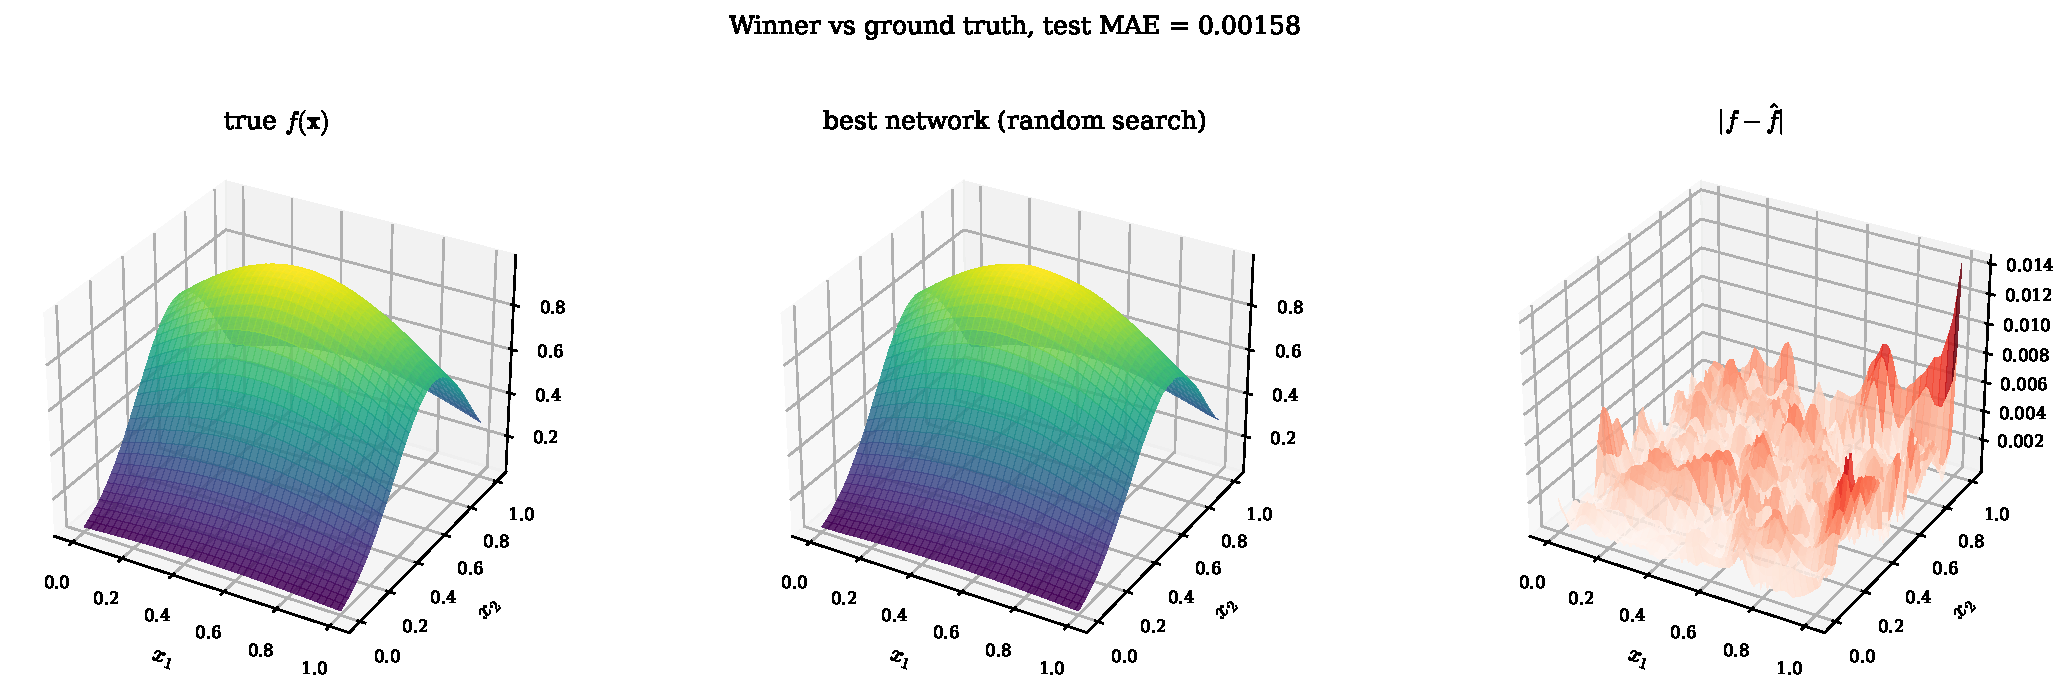
\includegraphics[width=0.92\linewidth]{figures/nas_best_surface.pdf}
\end{center}

\vspace{-0.2em}
{\footnotesize Stored teaching run of \texttt{03\_02}. Left to right: the true target, the winning configuration retrained from scratch (4L 256-224-128-256 relu lr 5.5e-04), and the absolute error on $[0,1]^2$. Test MAE 0.00158 against 0.00294 for the hand-picked baseline, on the 2,000 test points the search never saw.}
\end{frame}

% --- Slide 22b: the same search on a DEQN ---
\begin{frame}{The Same Search on a DEQN}
\small
A deep equilibrium net has no labels. A trial trains a policy network on the equilibrium
residual and returns an \emphc{Euler-equation error}; the search loop does not change.

\vspace{0.1cm}
\textbf{Model:} stochastic Brock--Mirman of Session 2 (\texttt{02\_02}): $\alpha=0.36$,
$\beta=0.99$, $\delta=0.1$, $\rho=0.9$, $\sigma=0.04$; savings rate through a sigmoid, five
Gauss--Hermite nodes, states drawn from the \texttt{02\_02} box. \textbf{Score:} mean
$|$relative Euler error$|$ on 4{,}096 held-out states after 3,000 episodes.
\textbf{Search space:} depth $\{1,2,3\}$, width $\{16,32,64,128\}$, relu / tanh, learning rate
log-uniform on $[10^{-4}, 10^{-2}]$; 30 random trials.

\vspace{0.1cm}
\begin{columns}[T]
\column{0.52\textwidth}
\begin{center}
\renewcommand{\arraystretch}{1.1}
{\scriptsize
\begin{tabular}{@{}lr@{}}
\toprule
 & mean $|$Euler error$|$ \\
\midrule
best trial: 3$\times$32 tanh, lr $2.0\cdot10^{-3}$ & $2.4\cdot10^{-4}$ \\
\texttt{02\_02} default: $2{\times}50$ relu, lr $3{\cdot}10^{-4}$ & $2.1\cdot10^{-3}$ \\
worst trial: 1$\times$16 relu, lr $1.6\cdot10^{-4}$ & $7.9\cdot10^{-3}$ \\
\bottomrule
\end{tabular}}
\end{center}
\column{0.44\textwidth}
\begin{center}
\renewcommand{\arraystretch}{1.1}
{\scriptsize
\begin{tabular}{@{}lr@{}}
\toprule
median score by level of & spread \\
\midrule
width & 3.5$\times$ \\
depth & 2.2$\times$ \\
learning rate, per decade & 1.5$\times$ \\
activation & 1.4$\times$ \\
\bottomrule
\end{tabular}}
\end{center}
\end{columns}
\vspace{0.05cm}
{\scriptsize Stored teaching run of \texttt{03\_02}, Section 7.}
\end{frame}

% --- Slide 23: Best Practices ---
\begin{frame}{Best Practices for NAS}
\small
\begin{columns}[T]
\column{0.50\textwidth}
\textbf{Search space design:}
\begin{itemize}
    \item Start small, expand if needed
    \item Use \emphc{log-scale} for learning rate
    \item Constrain to reasonable ranges
    \item Include the current best as a point
\end{itemize}

\vspace{0.3cm}
\textbf{Budget allocation:}
\begin{itemize}
    \item Count in epochs, not trials
    \item Run several seeds; report the range
    \item Successive halving: $\eta=3$, continue survivors
\end{itemize}

\column{0.47\textwidth}
\textbf{Common pitfalls:}
\begin{itemize}
    \item Search space too large $\Rightarrow$ wasted budget
    \item Ranking on the test set $\Rightarrow$ optimistic numbers; keep a holdout
    \item Best region on the boundary of a range $\Rightarrow$ widen it
    \item One seed $\Rightarrow$ a lottery ticket, not a result
\end{itemize}

\vspace{0.3cm}
\begin{alertblock}{Before searching}
Sweep each axis alone (\texttt{03\_01}, Section 3); fix the ones that do not move the error.
\end{alertblock}
\end{columns}
\end{frame}

% --- Slide 24: Connection to Economics ---
\begin{frame}{Connection to Economics}
\textbf{Where NAS matters in computational economics:}

\vspace{0.3cm}
\begin{enumerate}
    \item \textbf{Surrogate models:} Replace expensive simulations (e.g., climate IAMs) with NNs, architecture determines approximation quality.

    \vspace{0.2cm}
    \item \textbf{Policy functions:} Deep equilibrium nets (Session 2) approximate policy functions with a network. The search loop of \texttt{03\_02}, Section 7, runs unchanged with an Euler error as the score.

    \vspace{0.2cm}
    \item \textbf{High-dimensional problems:} As the state grows (Sessions 4 and 5), width and learning rate have to be re-tuned; a random search with a few seeds is the cheap way to do it.

    \vspace{0.2cm}
    \item \textbf{Reproducibility:} Automated search documents \emph{which} architectures were tried, making results more transparent than ``we chose 3 layers with 64 units.''
\end{enumerate}
\end{frame}

% --- Slide 25: Summary + References ---
\begin{frame}{Summary}
\begin{columns}[T]
\column{0.55\textwidth}
\textbf{Key takeaways:}
\begin{enumerate}
    \item Configuration choice moves the error by orders of magnitude; which knob depends on the problem, and the search tells you
    \item Random search beats grid search when most axes are inert, and only then
    \item Bayesian optimization buys sample efficiency at the price of sequential trials
    \item Successive halving spends the epoch budget where it pays; continue survivors, count epochs
    \item Rank on validation, report on test, run several seeds; the score can be an Euler error
\end{enumerate}

\column{0.42\textwidth}
\textbf{References:}
{\scriptsize
\begin{itemize}\itemsep0pt
    \item \emphc{Elsken, Metzen \& Hutter (2019)}: \emph{NAS: A Survey}, JMLR 20(55).
    \item Bergstra \& Bengio (2012). \emph{Random search.} JMLR 13.
    \item Li et al.\ (2018). \emph{Hyperband.} JMLR 18(185).
    \item Garnett (2023). \emph{Bayesian optimization.} CUP.
    \item Snoek et al.\ (2012). \emph{Practical Bayesian optimization.} NeurIPS.
\end{itemize}
}
\end{columns}

\end{frame}

\end{document}
